\documentclass[hidelinks,12pt]{article}
\usepackage[left=0.25cm,top=1cm,right=0.25cm,bottom=1cm]{geometry}
%\usepackage[landscape]{geometry}
\textwidth = 20cm
\hoffset = -1cm
\usepackage[utf8]{inputenc}
\usepackage[spanish,es-tabla]{babel}
\usepackage[autostyle,spanish=mexican]{csquotes}
\usepackage[tbtags]{amsmath}
\usepackage{nccmath}
\usepackage{amsthm}
\usepackage{amssymb}
\usepackage{mathrsfs}
\usepackage{graphicx}
\usepackage{subfig}
\usepackage{standalone}
\usepackage[outdir=./Imagenes/]{epstopdf}
\usepackage{siunitx}
\usepackage{physics}
\usepackage{color}
\usepackage{float}
\usepackage{hyperref}
\usepackage{multicol}
%\usepackage{milista}
\usepackage{anyfontsize}
\usepackage{anysize}
%\usepackage{enumerate}
\usepackage[shortlabels]{enumitem}
\usepackage{capt-of}
\usepackage{bm}
\usepackage{relsize}
\usepackage{placeins}
\usepackage{empheq}
\usepackage{cancel}
\usepackage{wrapfig}
\usepackage[flushleft]{threeparttable}
\usepackage{makecell}
\usepackage{fancyhdr}
\usepackage{tikz}
\usepackage{bigints}
\usepackage{scalerel}
\usepackage{pgfplots}
\usepackage{pdflscape}
\pgfplotsset{compat=1.16}
\spanishdecimal{.}
\renewcommand{\baselinestretch}{1.5} 
\renewcommand\labelenumii{\theenumi.{\arabic{enumii}})}
\newcommand{\ptilde}[1]{\ensuremath{{#1}^{\prime}}}
\newcommand{\stilde}[1]{\ensuremath{{#1}^{\prime \prime}}}
\newcommand{\ttilde}[1]{\ensuremath{{#1}^{\prime \prime \prime}}}
\newcommand{\ntilde}[2]{\ensuremath{{#1}^{(#2)}}}

\newtheorem{defi}{{\it Definición}}[section]
\newtheorem{teo}{{\it Teorema}}[section]
\newtheorem{ejemplo}{{\it Ejemplo}}[section]
\newtheorem{propiedad}{{\it Propiedad}}[section]
\newtheorem{lema}{{\it Lema}}[section]
\newtheorem{cor}{Corolario}
\newtheorem{ejer}{Ejercicio}[section]

\newlist{milista}{enumerate}{2}
\setlist[milista,1]{label=\arabic*)}
\setlist[milista,2]{label=\arabic{milistai}.\arabic*)}
\newlength{\depthofsumsign}
\setlength{\depthofsumsign}{\depthof{$\sum$}}
\newcommand{\nsum}[1][1.4]{% only for \displaystyle
    \mathop{%
        \raisebox
            {-#1\depthofsumsign+1\depthofsumsign}
            {\scalebox
                {#1}
                {$\displaystyle\sum$}%
            }
    }
}
\def\scaleint#1{\vcenter{\hbox{\scaleto[3ex]{\displaystyle\int}{#1}}}}
\def\bs{\mkern-12mu}


\usepackage{titling}
\setlength{\droptitle}{-3cm}
\title{Funciones ortogonales y Series de Fourier \\[0.3em]  \large{Material Complementario 01 - Técnica de separación de variables} \vspace{-3ex}}
\author{M. en C. Gustavo Contreras Mayén}
\date{ }



\begin{document}
\vspace{-2in}
\maketitle
\fontsize{14}{14}\selectfont
\tableofcontents
\newpage

% Dos vectores $\vb{A}$ y $\vb{B}$ son ortogonales si $\vb{A} \cdot \vb{B} = 0$. En forma de componentes, $\vb{A} = a_{i} \, \vu{e}_{i}$ y $\vb{B} = b_{i} \, \vu{e}_{i}$; $\vb{A}$ y $\vb{B}$ son ortogonales si $ a_{i} \, b_{i} = 0$.
% \par
% Se puede pensar en una función $A (x)$ como un vector. Si solo tres valores de $x$ son importantes, $x_{1}, x_{2}, x_{3}$, entonces los componentes de la función $A (x)$ (considerada como un vector) son:
% \begin{align*}
% A (x_{1}) \equiv a_{1}, \hspace{1cm}  (x_{2}) \equiv a_{2}, \hspace{1cm} A (x_{3}) \equiv a_{3}
% \end{align*}
% La función $A (x)$ es ortogonal a la función $B (x)$ (por definición) si $a_{i} \, b_{i} = 0$. Sin embargo, en problemas particulares, el dominio de las funciones $A(x)$ y $B(x)$ se define en $[0, L]$, por lo que todos los valores de $x$ entre $0$ y $L$ son importantes.
% \par
% \emph{La función $A (x)$ se puede considerar como un vector de dimensión infinita}, cuyas componentes son $A (x_{i})$ para todo $x_{i}$ en algún intervalo. De esta manera, se diría que la función $A (x)$ es ortogonal a $B (x)$ si $A (x_{i}) \, B (x_{i}) = 0$, donde están incluidos todos los puntos entre $0$ y $L$. Por lo tanto, es natural definir la función $A (x)$ para que sea ortogonal a $B (x)$ si:
% \begin{align*}
% \int_{0}^{L} A (x) \, B (x) \dd{x} = 0
% \end{align*}
% La integral reemplaza el producto escalar del vector; ambos son ejemplos de \enquote{productos internos}.
% \par
% En vectores, tenemos que los tres vectores unitarios son mutuamente perpendiculares (ortogonales) $\vu{i}, \vu{j}, \vu{k}$ conocidos como vectores base estándar. En forma de componentes:
% \begin{align*}
% \vb{A} = a_{1} \, \vu{i} + a_{2} \, \vu{j} + a_{3} \, \vu{k} 
% \end{align*}
% donde $a_{1}$ es la proyección de $\vb{A}$ en la dirección de $\vu{i}$, de la misma forma para las otras dos componentes.
% \par
% A veces deseamos representar $\vb{A}$ en términos de otros vectores mutuamente ortogonales (que pueden ser vectores no unitarios) $\vb{u}, \vb{v}, \vb{w}$, llamados conjunto ortogonal de vectores. Entonces:
% \begin{align*}
% \vb{A} = \alpha_{u} \, \vb{u} + \alpha_{v} \, \vb{v} + \alpha_{w} \, \vb{w}
% \end{align*}

% Para determinar las coordenadas $\alpha_{u}, \alpha_{v}, \alpha_{w}$ con respecto a este conjunto ortogonal, $\vb{u}, \vb{v}, \vb{w}$, podemos formar ciertos productos escalares. Por ejemplo:
% \begin{align*}
% \vb{A} \cdot \vb{u} = \alpha_{u} \, \vb{u} \cdot \vb{u} + \alpha_{v} \, \vb{v} \cdot \vb{u} + \alpha_{w} \, \vb{w} \cdot \vb{u}
% \end{align*}
% Como $\vb{v} \cdot \vb{u} = 0$ y $\vb{w} \cdot \vb{u} = 0$, ya que asumimos que este nuevo conjunto era mutuamente ortogonal. Por lo tanto, podemos resolver fácilmente la coordenada $\alpha_{u}$, de $\vb{A}$ en la dirección $u$:
% \begin{align}
% \alpha_{u} = \dfrac{\vb{A} \cdot {u}}{\vb{u} \cdot \vb{u}}
% \label{eq:ecuacion_03_45}
% \end{align}
% $\alpha_{u} \, \vb{u}$ es la proyección del vector $\vb{A}$ en la dirección $u$.
% \par
% Para las funciones, podemos hacer algo similar. Si $f (x)$ se puede representar mediante una combinación lineal del conjunto ortogonal, $\sin n \, \pi \, x / L$, entonces:
% \begin{align*}
% f(x) = \nsum_{n=1}^{\infty} B_{n} \, \sin \dfrac{n \, \pi \, x}{L}
% \end{align*}
% donde $B_{n}$ puede interpretarse como las coordenadas de $f (x)$ con respecto a la \enquote{dirección} (o vector base) $\sin n \, \pi \, x / L$. Para determinar estas coordenadas, tomamos el producto interno con una función de base arbitraria (vector) $\sin n \, \pi \, x / L$, donde el producto interno de dos funciones es la integral de su producto. Así, como antes:
% \begin{align*}
% \int_{0}^{L} f(x) \, \sin \dfrac{n \, \pi \, x}{L} \dd{x} = \nsum_{n=1}^{\infty} B_{n} \, \int_{0}^{L} \sin \dfrac{n \, \pi \, x}{L} \, \sin \dfrac{m \, \pi \, x}{L} \dd{x}
% \end{align*}
% Ya que $\sin \dfrac{n \, \pi \, x}{L}$ es un conjunto de funciones ortogonales:
% \begin{align*}
% \scaleint{6ex}_{\bs 0}^{L} \sin \dfrac{n \, \pi \, x}{L} \, \sin \dfrac{m \, \pi \, x}{L} \dd{x} = 0 \hspace{1.5cm} \mbox{para } n \neq m
% \end{align*}
% Por lo tanto, resolvemos para la coordenada (coeficiente) $B_{n}$:
% \begin{align}
% B_{n} = \dfrac{\displaystyle \int_{0}^{L} f(x) \, \sin \left(\dfrac{m \, \pi \, x}{L} \right) \dd{x}}{\displaystyle \int_{0}^{L} f(x) \, \sin^{2} \left( \dfrac{m \, \pi \, x}{L} \right) \dd{x}}
% \label{eq:ecuacion_03_46}
% \end{align}
% Consideremos que esta es la misma idea que la fórmula de proyección de la ec. (\ref{eq:ecuacion_03_45}). Tenemos que:
% \begin{align*}
% \int_{0}^{L} \sin^{2} \left( \dfrac{m \, \pi \, x}{L} \right) \dd{x} = \dfrac{L}{2}
% \end{align*}
% Por lo que la expresión para $B_{n}$ tiene la siguiente forma:
% \begin{align}
% B_{n} = \dfrac{2}{L} \, \int_{0}^{L} f(x) \, \sin \left(\dfrac{m \, \pi \, x}{L} \right) \dd{x}
% \label{eq:ecuacion_03_47}
% \end{align}
% Ambas expresiones (\ref{eq:ecuacion_03_45}) y (\ref{eq:ecuacion_03_46}) se dividen por algo. En la (\ref{eq:ecuacion_03_45}) es $\vb{u} \cdot \vb{u}$, o la longitud del vector $u$ al cuadrado. Por lo tanto:
% \begin{align*}
% \int_{0}^{L} \sin^{2} \left( \dfrac{m \, \pi \, x}{L} \right) \dd{x}
% \end{align*}
% puede considerarse como la longitud al cuadrado de $\sin  n \, \pi \, x / L$ (aunque aquí la \emph{longitud} no significa nada más que la raíz cuadrada de la integral). De esta manera, la longitud al cuadrado de la función $\sin  n \, \pi \, x / L$ es $L / 2$, lo cual es una explicación de la aparición del término $2 / L$ en la ec. (\ref{eq:ecuacion_03_47}).

%Ref. Echeverría - Apuntes de ED Cap. 6.

\section{Producto punto.}

En el curso de Álgebra Lineal se estudió el producto punto (o producto escalar) entre vectores en $\mathbb{R}^{n}$, por ejemplo, para $n = 3$, con los vectores $\vb{v} = (v_{1}, v_{2}, v_{3})$ y $\vb{u} = (u_{1}, u_{2}, u_{3})$, entonces:
\begin{align*}
\vb{v} \cdot \vb{u} = v_{i} \, u_{i}
%\label{eq:ecuacion_06_01_01}
\end{align*}

El producto punto es importante por varias razones:
\begin{enumerate}
\item  Se puede escribir la norma de un vector a través del producto punto:
\begin{align*}
\norm{\vu{u}} = \vb{u} \cdot \vb{u}
%\label{eq:ecuacion_06_01_02}
\end{align*}
\item  El ángulo entre dos vectores se calcula con la ayuda del producto punto como:
\begin{align*}
\cos \theta = \dfrac{\vb{u} \cdot \vb{u}}{\norm{\vb{u}} \, \norm{\vb{u}}}
%\label{eq:ecuacion_06_01_03}
\end{align*}
\item  La propiedad más importante del producto punto: permite hallar un vector como combinación lineal de una base fácilmente siempre y cuando la base fuera ortogonal. 
\end{enumerate}

Por ejemplo, si $v_{1}, v_{2}, v_{3}$ es una base de vectores en $\mathbb{R}^{3}$ entonces el vector $\vb{v}$ puede escribirse como combinación lineal de los vectores base:
\begin{align}
\vb{v} = c_{i} \, v_{i}
\label{eq:ecuacion_06_01_04}
\end{align}

Si los vectores son ortogonales entre sí, es decir:
\begin{align*}
v_{1} \cdot v_{2} = 0 \hspace{1cm} v_{1} \cdot v_{3} = 0  \hspace{1cm} v_{2} \cdot v_{3} = 0
%\label{eq:ecuacion_06_01_05}
\end{align*}
entonces para hallar los $c_{i}$ simplemente se toma el producto punto de la ec. (\ref{eq:ecuacion_06_01_04}). Por ejemplo, para hallar $c_{1}$ se toma el producto punto con $v_{1}$ usando la ec. (\ref{eq:ecuacion_06_01_04}):
\begin{align*}
\vb{v} \cdot v_{1} = c_{1} \, v_{1} \cdot v_{1} + c_{2} \, v_{2} \cdot v_{1} + c_{3} \, v_{3} \cdot v_{1} = c_{1} \, \norm{v_{1}}^{2}
%\label{eq:ecuacion_06_01_06}
\end{align*}
es decir:
\begin{align*}
c_{1} = \dfrac{\vb{v} \cdot v_{1}}{\norm{v_{1}}^{2}}
%\label{eq:ecuacion_06_01_07}
\end{align*}
de forma análoga se calcularían los coeficientes $c_{2}$ y $c_{3}$:
\begin{align*}
c_{2} = \dfrac{\vb{v} \cdot v_{2}}{\norm{v_{2}}^{2}} \hspace{1.5cm} c_{3} = \dfrac{\vb{v} \cdot v_{3}}{\norm{v_{3}}^{2}} 
%\label{eq:ecuacion_06_01_08}
\end{align*}

Lo más sorprendente del producto punto es que hay una generalización natural para las funciones, de modo que lo anterior siga siendo válido. Para ver cuál debe ser esa generalización, supongamos primero que los vectores son vectores infinitos, es decir:
\begin{align}
\begin{aligned}
\vb{v} &= (x_{1}, x_{2}, x_{3}, \ldots, x_{n}, \ldots) \\
\vb{u} &= (y_{1}, y_{2}, y_{3}, \ldots, y_{n}, \ldots)
\end{aligned}
\label{eq:ecuacion_06_01_09}
\end{align}
para tales vectores infinitos (de hecho son sucesiones) es natural definir el producto punto como:
\begin{align}
\vb{v} \cdot \vb{u} = x_{i} \, y_{i}
\label{eq:ecuacion_06_01_10}
\end{align}

Claramente, como en este caso el producto punto es una serie que no necesariamente converge, por lo que deben imponerse ciertas restricciones sobre los vectores para los cuales puede realizarse el producto punto anterior. 
\par
Ahora bien, una función $f(t)$ sobre un intervalo $[a, b]$ puede considerarse en cierto sentido como un vector infinito. Por ejemplo, si el intervalo fuera $[0, 1]$ la función $f(t)$ sería el vector con entradas $f(0), f(\frac{1}{10}), f(\frac{1}{\sqrt{2}}), \ldots, f(1)$, etc. La diferencia con el caso anterior, es que como el intervalo es un continuo no se pueden indicar las entradas en forma ordenada ya que en un intervalo entre dos puntos cualquiera, siempre aparece otro punto por lo que hay que buscar una versión continua de la serie de la ec. (\ref{eq:ecuacion_06_01_10}). 

\subsection{El producto interior.}

La integral puede verse como la versión continua de una serie, por lo que tiene sentido definir el producto punto entre dos funciones $f(t)$ y $g(t)$ como:
\begin{align}
f(t) \cdot g(t) = \int_{a}^{b} f(t) \, g(t) \dd{t}
\label{eq:ecuacion_06_01_11}
\end{align}

La definición anterior es la adecuada para generalizar el producto punto, sin embargo, es usual hacer unos cambios en la notación:
\begin{enumerate}
\item En vez de llamar a la operación producto punto se utiliza el nombre de \emph{producto interior}.
\item Como la notación puede confundirse con el producto ordinario de funciones, se modifica la notación a la notación \emph{bra-ket de Dirac}. 
\end{enumerate}

Básicamente, la notación bra-ket consiste en adornar las funciones para indicar que se va a realizar un producto interior entre ellas. De esta forma, se escribe una función $f(t)$ como $\ket{f(t)}$ donde los símbolos alrededor de la función sirven para recordar que se tiene la intención de tomar un producto interior (como veremos más adelante, la notación nos servirá para representar otras cantidades en mecánica cuántica). Por lo tanto,si se quiere realizar el producto interior entre $\ket{f(t)}$ y $\ket{g(t)}$, se le da \enquote{vuelta} a una de los funciones, por ejemplo, se cambia $\ket{f(t)}$ por $\bra{f(t)}$ y de esta forma la ec. (\ref{eq:ecuacion_06_01_11} se escribe:
\begin{align}
\braket{f(t)}{g(t)} \equiv \int_{a}^{b} f(t) \, g(t) \dd{t}
\label{eq:ecuacion_06_01_12}
\end{align}
esta notación da una mejor explicación al nombre producto interior pues las funciones $f(t), g(t)$ quedan dentro (en el interior) de $< >$. Con esta nueva notación,las propiedades usuales del producto punto se siguen cumpliendo.

\subsection{Propiedades del producto interior.}

Si $\ket{f(t)}$ y $\ket{g(t)}$ son dos funciones definidas sobre el intervalo $[a, b]$ el producto interior de $\ket{f(t)}$ con $\ket{g(t)}$ se define como:
\begin{align}
\braket{f(t)}{g(t)} \equiv \int_{a}^{b} f(t) \, g(t) \dd{t}
\label{eq:ecuacion_06_10_13}
\end{align}

Algunas propiedades del producto interior son:
\begin{enumerate}[label=\roman*)]
\item Conmutatividad:
\begin{align}
\braket{f(t)}{g(t)} = \braket{g(t)}{f(t)}
\label{eq:ecuacion_06_01_14}
\end{align}
\item Linealidad: Si $\ket{h(t)}$ es otra función y $c \in \mathbb{R}$ una constante, entonces si se representa $g(t) + c \, h(t)$ como $\ket{g(t) + c \, h(t)}$:
\begin{align}
\braket{f(t)}{g(t) + c \, h(t)} = \braket{f(t)}{g(t)} + c \, \braket{f(t)}{h(t)}
\label{eq:ecuacion_06_01_15}
\end{align}
\item Norma de una función: La norma de una función $\ket{f(t)}$ se define como:
\begin{align}
\norm{f(t)}^{2} = \braket{f(t)}{f(t)} = \int_{a}^{b} [f(t)]^{2} \dd{t}
\label{eq:ecuacion_01_06_16}
\end{align}
\item Ángulo entre funciones: El ángulo entre dos funciones $\ket{f(t)}$, $\ket{g(t)}$ se define como:
\begin{align}
\cos \theta = \dfrac{\braket{f(t)}{g(t)}}{\norm{f(t)} \, \norm{g(t)}}
\label{eq:ecuacion_06_01_17}
\end{align}
\item Ortogonalidad de funciones: Las funciones $\ket{f(t)}$, $\ket{g(t)}$ son ortogonales si su producto interior es cero, es decir:
\begin{align}
\braket{f(t)}{g(t)} = \int_{a}^{b} f(t) \, g(t) \dd{t} = 0
\label{eq:ecuacion_06_01_18}
\end{align}
\end{enumerate}

En la teoría de funciones hay muchas familias de funciones ortogonales. Sin embargo, para la teoría de Fourier hay una familia particularmente importante, que es la familia de \emph{funciones sinusoidales}, es decir, la familia de senos y cosenos cuya frecuencia es un múltiplo de una frecuencia fundamental. Antes de ver que tal familia es ortogonal, recordemos el concepto de función periódica.

\section{Función periódica.}

Una función $f(t)$ es periódica de período $T > 0$ si para todo $t$ se tiene:
\begin{align}
f(t + T) = f(t)
\label{eq:ecuacion_06_01_19}
\end{align}

Algunas funciones conocidas que son periódicas son senos, cosenos (que son de período $2 \, \pi$ y como caso límite las funciones constantes (que serían funciones con cualquier período.
\par
Otra propiedad de una función periódica es que si $T$ es un período para la función entonces $2 \, T$, $3 \, T$, también son períodos según la definición, por lo que el período no es único. Sin embargo, el valor menor de $T$ que cumpla con la ec. (\ref{eq:ecuacion_06_01_19}) se llama generalmente el \emph{período fundamental}.
\par
Una propiedad inmediata de la interpretación de la integral como el área bajo la curva o simplemente a partir de un cambio de variable, es que la integral de una función sobre intervalos de longitud $T$ siempre devuelve el mismo valor, es decir: Si $f(t)$ es una función con período $T$ entonces para cualquier $a$, $b$ se tiene que:
\begin{align*}
\int_{a}^{a+T} f(t) \dd{t} = \int_{b}^{b+T} f(t) \dd{t}
%\label{eq:ecuacion_06_01_20}
\end{align*}
Esto significa que si $f(t)$ es una función definida sobre toda la recta real con período $T$, entonces se puede estudiar la función alrededor de un intervalo simétrico con respecto al origen, por ejemplo, el intervalo $\bigg[-\dfrac{T}{2}, \dfrac{T}{2} \bigg]$. Más aún, por el momento es suficiente pensar que las funciones tienen un período $2 \, \pi$, pues de lo contrario, puede hacerse un reescalamiento para que sea de período $2 \, \pi$. Por ejemplo, si $f(t)$ es de período $T$ se puede definir:
\begin{align*}
g(t) \equiv f \left( \dfrac{T}{2 \, \pi} \right)
%\label{eq:ecuacion_06_01_21}
\end{align*}
y $g(t)$ es de período $2 \, \pi$ porque:
\begin{align*}
g(t + 2 \, \pi) = f \left( \dfrac{T}{2 \, \pi} (t + 2 \, \pi) \right) = f \left( \dfrac{T \, t}{2 \, \pi} + T \right) = f \left( \dfrac{T \, t}{2 \, \pi} \right) = g(t)
%\label{eq:ecuacion_06_01_22}
\end{align*}

Es decir, si $f(t)$ es una función de período $T$, entonces:
\begin{align*}
g(t) \equiv f \left( \dfrac{T}{2 \, \pi} \, t \right)
%\label{eq:ecuacion_06_01_23}
\end{align*}
es una función de período $2 \, \pi$.
\par
Por lo tanto, se puede estudiar sin pérdida de generalidad las funciones de período $2 \, \pi$. Como se dijo antes,las funciones más importantes para las series de Fourier son las funciones sinusoidales, es decir, expresiones de la forma:
\begin{align*}
\sin (\omega \, t) \hspace{1.5cm} \cos (\omega \, t)
%\label{eq:ecuacion_01_01_24}
\end{align*}
donde $\omega$ es la frecuencia angular y el período es:
\begin{align*}
T = \dfrac{2 \, \pi}{\omega}
%\label{eq:ecuacion_06_01_25}
\end{align*}

\section{Serie de Fourier.}

La idea de una serie de Fourier es que cualquier función periódica (que cumpla ciertas condiciones matemáticas) puede descomponerse como una serie infinita de senos y cosenos. Para dar una idea general antes de entrar en detalle, supongamos que se tiene la función $f(t) = t$ definida sobre $[-\pi, \pi]$  y luego se extiende periódicamente tal como se indica en la siguiente figura (\ref{fig:06_01_01}).
 \begin{figure}[H]
     \centering
     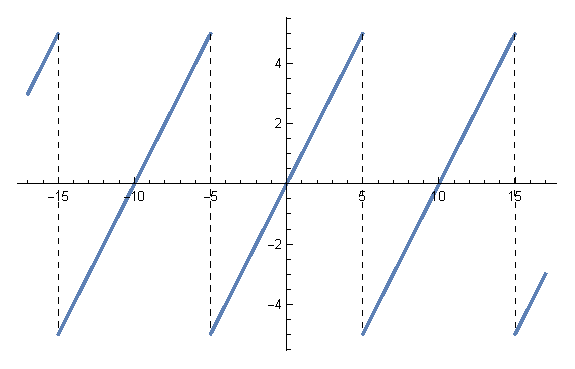
\includegraphics[scale=1]{Imagenes/Funciones_Ortogonales_01.eps}
     \caption{La función $f(t) = t$, por su forma se le conoce también como diente de sierra.}
     \label{fig:06_01_01}
 \end{figure}
 La idea de las series de Fourier es aproximar la función por sumas de senos y cosenos. Por ejemplo, pronto se verá que la serie de Fourier para la función anterior es:
 \begin{align}
f(t) = \nsum_{n=1}^{\infty} \dfrac{2 \, (-1)^{n+1}}{n} \, \sin (n \, t)
\label{eq:ecuacion_01_06_26}
 \end{align}
Las siguientes figuras (\ref{fig:06_01_02}) ilustran la función $f(t)$ junto con las primeras sumas parciales con $ n = 1, 2, 3, 5, 10, 100$.
\begin{figure}[H]
    \centering
    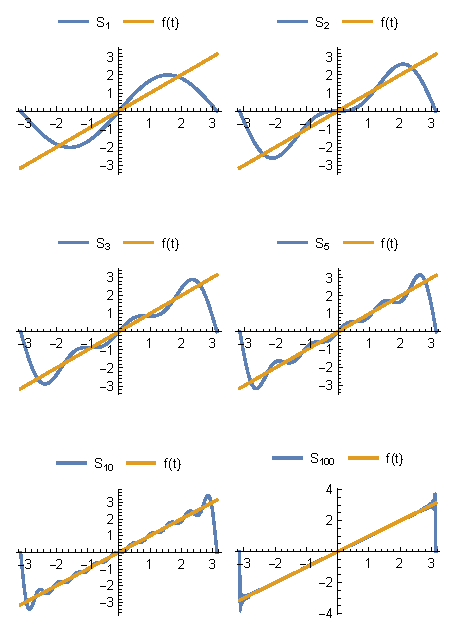
\includegraphics[scale=1.5]{Imagenes/Funciones_Ortogonales_02.eps}
    \caption{La función $f(t) = t$ y las funciones obtenidas mediante el desarrollo de Fourier, el subíndice en $S_{i}$ indica el número de términos incluidos en la suma.}
    \label{fig:06_01_02}
\end{figure}

Se puede observar que a medida de que aumentan los términos en las sumas parciales, la aproximación es cada vez mejor a la función original, sin embargo, en los extremos de la función, que corresponden a los puntos en que es discontinua, pareciera que la serie de Fourier no se aproxima bien a la función original. Tal fenómeno se conoce como el \emph{fenómeno de Gibbs}, aunque no se revisará en este momento, es bueno saber que ocurre cerca de los puntos de discontinuidad de la función.

\subsection{Funciones ortogonales.}

Revisaremos que las funciones $\ket{1}$ (es decir la función constante igual a $1$, $\ket{cos (nt)}$, $\ket{\sin (nt)}$ son ortogonales sobre el intervalo $[- \pi, \pi]$. Calculemos inicialmente la norma de cada una de las funciones:
\begin{align*}
\norm{1}^{2} = \braket{1}{1} = \int_{-\pi}^{\pi} \dd{t} = 2 \,\pi
%\label{eq:ecuacion_06_01_29}
\end{align*}

Para calcular la norma del seno y del coseno:
\begin{align*}
\norm{\cos (nt)}^{2} &= \braket{\cos(nt)}{\cos(nt)} = \int_{-\pi}^{\pi} \cos^{2} (nt) \dd{t} = \pi %\label{eq:ecuacion_06_01_30}
\\[0.5em]
\norm{\sin (nt)}^{2} &= \braket{\sin(nt)}{\sin(nt)} = \int_{-\pi}^{\pi} \sin^{2} (nt) \dd{t} = \pi %\label{eq:ecuacion_06_01_31}
\end{align*}

La ortogonalidad de $\ket{1}$, $\ket{cos (nt)}$, $\ket{\sin (nt)}$ es clara al ocupar la definición de la integral como el área bajo la curva:
\begin{align*}
\braket{1}{\cos (nt)} &= \int_{-\pi}^{\pi} \cos (nt) \dd{t} = 0 %\label{eq:ecuacion_06_01_32}
\\[0.5em]
\braket{1}{\sin (nt)} &= \int_{-\pi}^{\pi} \sin (nt) \dd{t} = 0 %\label{eq:ecuacion_06_01_33}
\end{align*}

Para la ortogonalidad del seno con el coseno se pueden utilizar su representación compleja:
\begin{align*}
\braket{\cos{nt}}{\sin(nt)} = \int_{-\pi}^{\pi} \left( \dfrac{e^{int} + e^{-int}}{2} \right) \left( \dfrac{e^{imt} + e^{-imt}}{2} \right) \dd{t} = 0
%\label{eq:ecuacion_06_01_34}
\end{align*}
de manera análoga se demuestra que:
\begin{align*}
%\begin{aligned}
\braket{\sin(nt)}{\sin(mt)} &= 0 \\[0.5em]
\braket{\sin(nt)}{\cos(mt)} &= 0 \\[0.5em]
\braket{\sin(nt)}{\cos(nt)} &= 0
%\end{aligned}
%\label{eq:ecuacion_06_01_35}
\end{align*}

Concluimos que el conjunto de funciones $\left\{ \ket{1}, \ket{\cos(nt)}, \ket{\sin(nt)} \right\}$ con $n \in \mathbb{N}$ son ortogonales entre sí, en el intervalo $[-\pi, \pi]$.
Nuevamente, la idea de las series de Fourier es que las funciones anteriores \emph{forman una base para las funciones periódicas}, es decir, si $f(t)$ es una función periódica de período $2 \, \pi$, entonces $f(t)$ se puede expandir como:
\begin{align}
\ket{f(t)} = \dfrac{a_{0}}{2} \ket{1} + \nsum_{n=1}^{\infty} \big( a_{n} \, \ket{\cos (n \, t)} + b_{n} \, \ket{\sin (n \, t)} \ \big)
\label{eq:ecuacion_06_01_38}
\end{align}
donde $a_{0}, a_{n}, b_{n}$ son coeficientes por determinar (el factor $\frac{1}{2}$ de $a_{0}$ es una convención usual). Para hallar los coeficientes se utiliza la ortogonalidad de las funciones\footnote{Presentamos un desarrollo general, aunque una demostración estricta requiere de más elementos, que se pueden consultar en los textos tanto de cálculo como de álgebra lineal.}.
\par
Por ejemplo, para determinar el coeficiente $a_{0}$ se aplicamos $\ket{1}$ en ambos lados de la ec. (\ref{eq:ecuacion_06_01_38}), para obtener:
\begin{align}
\braket{1}{f(t)} = \dfrac{a_{0}}{2} \braket{1}{1} + \nsum_{n=1}^{\infty} \big( a_{n} \, \braket{1}{\cos (n \, t)} + b_{n} \, \braket{1}{\sin (n \, t)} \ \big)
\end{align}
por lo que:
\begin{align}
\braket{1}{f(t)} = \pi \, a_{0}
\label{eq:ecuacion_06_01_40}
\end{align}
o bien:
\begin{align}
a_{0} = \dfrac{1}{\pi} \, \braket{1}{f(t)} = \dfrac{1}{\pi} \, \int_{-\pi}^{\pi} f(t) \dd{t}
\label{eq:ecuacion_06_01_41}
\end{align}

Para hallar $a_{m}$ se aplica $\bra{\cos (mt)}$ en ambos lados de la ec. (\ref{eq:ecuacion_06_01_38}):
\begin{align}
\begin{aligned}
\braket{\cos(m \, t)}{f(t)} &= \dfrac{a_{0}}{2} \braket{\cos(m \, t)}{1} + \nsum_{n=1}^{\infty} \bigg[ a_{m} \, \braket{\cos (m \, t)}{\cos (n \, t)} + \\[0.5em]
&+ b_{n} \, \braket{\cos (m \, t)}{\sin (n \, t)} \bigg]
\end{aligned}
\label{eq:ecuacion_06_01_42}
\end{align}
de las relaciones encontradas previamente, la expresión se reduce a:
\begin{align}
\braket{\cos(m \, t)}{f(t)} = a_{m} \, \braket{\cos (n \, t)}{\cos (n \, t)} = \pi \, a_{m}
\label{eq:ecuacion_06_01_43}
\end{align}
renombrando nuevamente el subíndice:
\begin{align}
a_{n} = \dfrac{1}{\pi} \, \braket{\cos (n \, t)}{f(t)} = \dfrac{1}{\pi} \, \int_{-\pi}^{\pi} \cos (n \, t) \, f(t) \dd{x}
\label{eq:ecuacion_06_01_44}
\end{align}
De forma análoga se tiene que:
\begin{align}
b_{n} = \dfrac{1}{\pi} \, \braket{\sin (n \, t)}{f(t)} = \dfrac{1}{\pi} \, \int_{-\pi}^{\pi} \sin (n \, t) \, f(t) \dd{x}
\label{eq:ecuacion_06_01_45}
\end{align}

\subsection{Serie de Fourier de una función \texorpdfstring{$f(t)$}{f(t)}.}

Si una función $f(t)$ es una función definida en el intervalo $[-\pi, \pi]$, la serie de Fourier asociada a la función es:
\begin{align}
f(t) \approx \dfrac{a_{0}}{2} + \nsum_{n=1}^{\infty} \big( a_{n} \, \cos (n \, t) + b_{n} \, \sin (n \, t) \big)
\label{eq:ecuacion_06_01_46}
\end{align}
donde:
\begin{align}
a_{0} &= \dfrac{1}{\pi} \, \int_{-\pi}^{\pi} f(t) \dd{t} \label{eq:ecuacion_06_01_47} \\[0.5em]
a_{n} &= \dfrac{1}{\pi} \, \int_{-\pi}^{\pi} \cos (n \, t) \, f(t) \dd{t} \label{eq:ecuacion_06_01_48} \\[0.5em]
b_{n} &= \dfrac{1}{\pi} \, \int_{-\pi}^{\pi} \sin (n \, t) \, f(t) \dd{t} \label{eq:ecuacion_06_01_49}
\end{align}

\textbf{Ejemplo. } La serie de Fourier para $f(t) = t$ en el intervalo $[-\pi, \pi]$.

Basta con calcular los coeficientes $a_{0}, a_{n}, b_{n}$, ocupando las expresiones (\ref{eq:ecuacion_06_01_47}), (\ref{eq:ecuacion_06_01_48}) y (\ref{eq:ecuacion_06_01_49}):
\begin{align*}
a_{0} &= \dfrac{1}{\pi} \int_{-\pi}^{\pi} t \dd{t} = 0 \\[0.5em]
a_{n} &= \dfrac{1}{\pi} \, \int_{-\pi}^{\pi} t \, \cos (n \, t) \dd{t} = 0 \\[0.5em]
b_{n} &= \dfrac{1}{\pi} \, \int_{-\pi}^{\pi} t \, \sin (n \, t) \dd{t} = \dfrac{2(-1)^{n+1}}{n}
\end{align*}
por lo que la serie de Fourier para $f(t) = t$, es:
\begin{align*}
f(t) \approx \nsum_{n=1}^{\infty} \dfrac{2(-1)^{n+1}}{n} \, \sin (n \, t)
\end{align*}

Es importante tener presente las condiciones matemáticas que garantizan que una función sea igual a su serie de Fourier asociada (el teorema es exactamente igual sobre cualquier intervalo, por lo que se presenta únicamente sobre $(-\pi, \pi)$.
\par
Supongamos que $f(t)$ es derivable y $f(t)$, $\ptilde{f}$  son funciones continuas por partes. Entonces la serie de Fourier asociada a $f$ converge a $f(t)$ en todo punto de continuidad de $f$. En un punto de discontinuidad, la serie converge al promedio, es decir:
\begin{align}
\dfrac{f(t+) + f(t-)}{2}
\label{eq:ecuacion_06_01_55}
\end{align}

\textbf{Ejemplo. } Calcula la serie de Fourier para la función en partes:
\begin{align*}
f(x) = \begin{cases}
0 & -\pi < x < 0 \\
\pi - x, & 0 \leq x < \pi
\end{cases}
\end{align*}
En la figura (\ref{fig:06_01_03}) se presenta la gráfica
\begin{figure}[H]
    \centering
    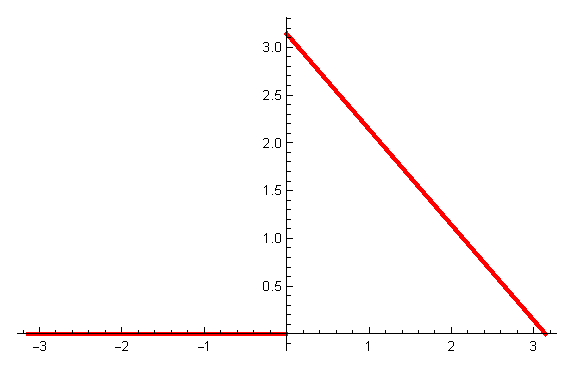
\includegraphics[scale=1]{Imagenes/Funciones_Ortogonales_03.eps}
    \caption{Gráfica de la función en partes.}
    \label{fig:06_01_03}
\end{figure}

Se revisa inicialmente la discontinuidad en el origen, por lo que en ese punto la serie de Fourier debe de converger a:
\begin{align*}
\dfrac{f(0+) + f(0-)}{2} = \dfrac{\pi}{2}
\end{align*}
De esta forma los coeficientes para la serie de Fourier, son:
\begin{align*}
a_{0} &= \dfrac{1}{\pi} \int_{-\pi}^{\pi} f(x) \dd{x} = \\[0.5em]
&= \dfrac{1}{\pi} \int_{0}^{\pi} (\pi - x) \dd{x} = \dfrac{\pi}{2}
\end{align*}
Para el coeficiente $a_{n}$:
\begin{align*}
a_{n} &= \dfrac{1}{\pi} \int_{-\pi}^{\pi} (\pi - x) \, \cos (n \, x) \dd{x} = \dfrac{1 - (-1)^{n}}{n^{2} \, \pi}
\end{align*}
y para el coeficiente $b_{n}$:
\begin{align*}
b_{n} &= \dfrac{1}{\pi} \int_{-\pi}^{\pi} (\pi - x) \, \sin (n \, x) \dd{x} = \dfrac{1}{n}
\end{align*}
Por lo que la expresión en serie de Fourier para $f(x)$ es:
\begin{align*}
f(x) = \dfrac{\pi}{4} + \nsum_{n=1}^{\infty} \bigg[ \dfrac{1 - (-1)^{n}}{n^{2} \, \pi} \, \cos (n \, x) + \dfrac{1}{n} \, \sin (n \, x) \bigg]
\end{align*}
En la figura (\ref{fig:06_01_04}) se muestra la función $f(x)$ y la serie de Fourier con términos $n = 1, 5, 10, 100$.
\begin{figure}[H]
    \centering
    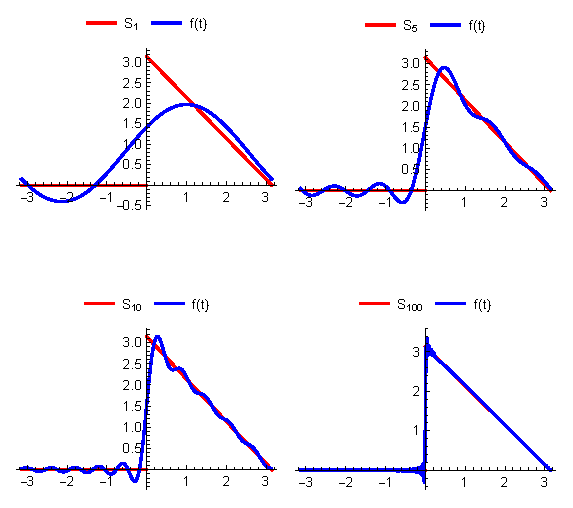
\includegraphics[scale=1.5]{Imagenes/Funciones_Ortogonales_04.eps}
    \caption{Series de Fourier para la función $f(x)$ en partes, el subíndice en $S_{i}$ indica el número de términos en la suma.}
    \label{fig:06_01_04}
\end{figure}

\subsection{Serie de Fourier de funciones pares e impares.}

No es necesario definir una función auxiliar para hallar la serie de Fourier, se puede desarrollar directamente a partir de la función original. Si $f(t)$ tiene período $T$, su semiperíodo es $p = \dfrac{T}{2}$.
\par
La serie de Fourier de una función definida en el intervalo $(-p, p)$ es:
\begin{align}
f(t) = \dfrac{a_{0}}{2} + \nsum_{n=1}^{\infty} \bigg[ a_{n} \, \cos \left( \dfrac{n \, \pi}{p} \, t \right) + b_{n} \, \sin \left( \dfrac{n \, \pi}{p} \, t \right) \bigg]
\label{eq:ecuacion_06_01_68}
\end{align}
donde los coeficientes son:
\begin{align}
\begin{aligned}
a_{0} &= \dfrac{1}{p} \, \int_{-p}^{p} f(t) \dd{t} \\[0.5em]
a_{n} &= \dfrac{1}{p} \, \int_{p}^{p} f(t) \, \cos \left( \dfrac{n \, \pi}{p} \, t \right) \dd{t} \\[0.5em]
b_{n} &= \dfrac{1}{\pi} \, \int_{-\pi}^{\pi} f(t) \, \sin \left( \dfrac{n \, \pi}{p} \, t \right) \dd{t}
\end{aligned}
\label{eq:ecuacion_06_01_69}
\end{align}

En el caso en que la función sea par o impar los coeficientes toman una forma más sencilla todavía.
\par
Una función es par si $f(t) = f(- t)$, es decir, su gráfica posee simetría con respecto al eje $y$. Una función es impar si $f(t) = -f(- t)$, su gráfica es simétrica con respecto al origen. Las funciones pares e impares poseen las siguientes propiedades:
\begin{enumerate}[label=\roman*)]
\item El producto de dos funciones pares es par.
\item El producto de dos funciones impares es par.
\item El producto de una función par y una función impar es impar.
\item Si $f(t)$ es una función par:
\begin{align*}
\int_{-p}^{p} f(t) \dd{t} = 2 \int_{0}^{p} f(t) \dd{t}
\end{align*}
\item Si $f(t)$ es una función impar:
\begin{align*}
\int_{-p}^{p} f(t) \dd{t} = 0
\end{align*}    
\end{enumerate}

Por ejemplo, si $f(t)$ es una función par, entonces los coeficientes de Fourier toman la forma:
\begin{align}
\begin{aligned}
a_{0} &= \dfrac{2}{p} \int_{0}^{p} f(t) \dd{t} \\[0.5em]
a_{n} &= \dfrac{2}{p} \int_{0}^{p} f(t) \, \cos \left( \dfrac{n \, \pi}{p} \, t \right) \dd{t} \\[0.5em]
b_{n} &= 0
\end{aligned}
\label{eq:ecuacion_06_01_70}
\end{align}

Por otro lado, si $f(t)$ es una función impar entonces los coeficientes de Fourier son:
\begin{align}
\begin{aligned}
a_{0} &= 0 \\[0.5em]
a_{n} &= 0 \\[0.5em]
b_{n} &= \dfrac{2}{p} \int_{0}^{p} f(t) \, \sin \left( \dfrac{n \, \pi}{p} \, t \right) \dd{t}
\end{aligned}
\label{eq:ecuacion_06_01_71}
\end{align}

En los casos anteriores la serie de Fourier se llama: \emph{serie de Fourier coseno} y \emph{serie de Fourier seno} respectivamente.

Si $f(t)$ es una función par su serie de Fourier se llama serie de Fourier coseno y viene dada por:
\begin{align}
f(t) = \dfrac{a_{0}}{2} + \nsum_{n=1}^{\infty} a_{n} \, \cos \left( \dfrac{n \, \pi}{p} \, t \right)
\label{eq:ecuacion_06_01_72}
\end{align}
donde:
\begin{align}
\begin{aligned}
a_{0} &= \dfrac{2}{p} \, \int_{0}^{p} f(t) \dd{t} \\[0.5em]
a_{n} &= \dfrac{2}{p} \int_{0}^{p} f(t) \, \cos \left( \dfrac{n \, \pi}{p} \, t \right) \dd{t} 
\end{aligned}
\label{eq:ecuacion_06_01_73}
\end{align}

% n= a = 2 p p f(tdt a n = 2 ( p p f(t cos nπ p t dt En el caso de que p = π la serie se simplifica en donde (6..73 f(t = a 2 + a n cos (nt (6..74 a n = 2 π a = 2 π π n= π f(tdt f(t cos(nt dt (6..75 

Si $f(t)$ es una función impar su serie de Fourier se llama la serie de Fourier seno, se expresa como:
\begin{align}
f(t) = \nsum_{n=1}^{\infty} b_{n} \, \sin \left( \dfrac{n \, \pi}{p} \, t \right)
\label{eq:ecuacion_06_01_76}
\end{align}
donde:
\begin{align}
b_{n} = \dfrac{2}{p} \int_{0}^{p} f(t) \, \sin \left( \dfrac{n \, \pi}{p} \, t \right) \dd{t}
\label{eq:ecuacion_06_01_77}
\end{align}

%en el caso en que p = π la serie se simplifica como f(t = ( nπ f(tsin p t dt (6..77 b n sin (nt (6..78 n= donde b n = 2 π ˆ π f(tsin(nt dt (6..79 A veces se quiere desarrollar una función que está definida únicamente sobre [,π] (o en el caso más general [,p] comounaseriedefourier.unaestrategiaesextenderla función arbitrariamente sobre todo el intervalo [ π, π] (o bien [ p, p] para obtener la serie de Fourier de la extensión. Obviamente, no todas las extensiones son igualmente útiles, en particular hay tres extensiones distintas que resultan igualmente útiles. Extensión par de la función: sereflejaf(t con respecto al eje y la función. Generalmente la extensión periódica se denota nuevamente como f(t por lo que se tiene el desarrollo de cosenos f(t = a 2 + ( nπ a n cos p t (6..8 n= 28

% 282 6 Ecuaciones Diferenciales en Derivadas Parciales donde a = 2 p p f(tdt a n = 2 ( p p f(tcos nπ p t dt (6..8 como se ve del cálculo de coeficientes, en la práctica la integral solo tiene que calcularse sobre el intervalo en el que está definida inicialmente la función por lo que no es necesario escribir la extensión explícitamente. Figura 6..6: Extensión par de la función Extensión impar de la función: sereflejalafunciónf(t con respecto al origen. En este caso se tiene el desarrollo de senos de la función ( nπ f(t = b n sin p t (6..82 n= donde b n = 2 p ˆ p ( nπ f(tsin p t dt (6..83 282

% 283 6 Ecuaciones Diferenciales en Derivadas Parciales Figura 6..7: Extensión impar de la función Extensión periódica de la función: Ahora se extiende la función de modo que tenga período p, esdecir,f(t + p =f(t. Enestecasolafuncióntienesemiperíodo p 2 por lo que se puede usar 6..68 y 6..69 con el cuidado de que se reemplaza p por p 2,esdecir, donde f(t = a 2 + n= ( ( ( 2nπ 2nπ a n cos p t + b n sin p t (6..84 a n = 2 p b n = 2 p p 2 p 2 a = 2 p p 2 p f(tdt= 2 p p f(tdt 2 f(tcos( 2nπ p t dt = 2 p p 2 f(tsin( 2nπ p p t dt = 2 p 2 p ( f(tcos 2nπ p t dt ( p f(tsin 2nπ p t dt (6..85 donde para la última igualdad se usó la propiedad de que la integral de una función periódica sobre intervalos de la misma longitud es igual. 283



\end{document}